\section{The Guardian of the Threshold}

\begin{quotex}
Thou austere and remorseless Hierophant,—thou who hast sought to convert to our brotherhood every spirit that seemed to thee most high and bold,—even thou knowest, by horrible experience, how vain the hope to banish FEAR from the heart of woman, \flright{\textsc{Edward Bulwer-Lytton}, \emph{Zanoni}}

\end{quotex}
There are two awakenings of Adam:

\paragraph{Awakening from the Muck}
\begin{quotex}
then the Lord God formed man of dust from the ground, and breathed into his nostrils the breath of life; and man became a living being. \flright{\textsc{Genesis 2:7}}

\end{quotex}

Since the mist watered the face of the earth, the dust was moist like mud. Hence Adam was composed of the elements of earth, water, and air as well as life. When Adam awoke, he saw it was good for him. He names the animals, which means he knew their essences and their purposes.

Moreover, since the world has an outside as well as an inside, Saint Basil the Great has a deeper understanding of the command to ``rule" the animals. He claimed that the animals represent various emotional states, which must be ``ruled" by the Intellect. The hylic man is more impressed by physical mastery of wild animals; on the other hand, the spiritual man is more impressed by the ability to master the emotions.

Similarly, Adam did not see God with human eyes. Valentin Tomberg explains how that could be possible:

\begin{quotex}
In the sixteenth century St. John of the Cross wrote in his work The Night of the Spirit and the Night of the Senses that light as such is invisible. It becomes visible by virtue of the many particles and larger and smaller objects that offer resistance to light on its path. Thus we see the sun's rays because the sun's light falls upon the ``atoms" of dust and illumines them. The same holds true for the light of the spirit. As such it is dark, but when it falls upon something—such as the problems and riddles of existence — it becomes visible and illumines them by effecting insight and understanding. \flright{\textsc{Valentin Tomberg}, \emph{Covenant of the Heart}}

\end{quotex}
This means that whenever Adam had a question, he could rely on God's grace to make the answer available to him in his interiority. Adam knew the animals, his own soul, the structure and purpose of the cosmos, and, most importantly, he knew God.

\emph{Thus Adam was one who knows.}

\paragraph{Awakening to Eve}
\begin{quotex}
So the Lord God caused a deep sleep to fall upon the man, and while he slept took one of his ribs and closed up its place with flesh; and the rib which the Lord God had taken from the man he made into a woman and brought her to the man. \flright{\textsc{Genesis 2:21-22}}

\end{quotex}
There was one riddle in particular. Adam could see the animals, who always acted out of instinct. There was nothing evil to see. Adam, on the other hand, was able to choose his actions. Thus, the cosmos was moral, but how could it be moral without a real choice. Therefore, he was given one law: not to eat of the tree of the knowledge of good and evil. There was no specific evil that he was commanded to avoid, but rather the very possibility of knowing evil.

\begin{wrapfigure}{rt}{.3\textwidth}
 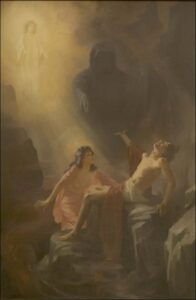
\includegraphics[scale=2]{a20200930TheGuardianoftheThreshold-img001.jpg} 
\caption{Dweller of the Threshold}
\end{wrapfigure}

There was something else amiss. Although Adam knew the animals, they did not know him. Therefore, none of them was a suitable companion for him. Since Adam knew his own soul, he could see clearly that a significant part of him, actually the most significant part, was missing in the world. That would be his companion.

Adam's deep sleep was a descent into his subconscious, to experience the submerged image of his Lover. When Adam awoke, he recognized Eve at once as his companion, wife and lover.

\emph{Thus Adam was one who loves.}

\paragraph{The Cherubim Block the Way}
\begin{quotex}
He drove out the man; and at the east of the garden of Eden he placed the cherubim, and a flaming sword which turned every way, to guard the way to the tree of life. \flright{\textsc{Genesis 3:24}}

\end{quotex}
As mentioned above, Adam could turn to the light of the Spirit whenever he had a question. At some point, he turned away from the Spirit, and looked elsewhere for understanding. There was darkness where there should have been light. The serpent inhabited that darkness and Adam turned to Eve, instead of to God, for advice. Together, since their souls were entangled, they ate the fruit of the tree.

Immediately, they saw evil and could not unsee it. They descended into the biological life of the animals: birth, life, and death. God sent angels to prevent a return to the Garden. They had to await the Redeemer who would break the cycle of the Ouroboros.

\paragraph{The Dweller of the Threshold}

In the novel \emph{Zanoni}, Edward Bulwer-Lytton describes the situation of two initiates, Mejnour and Zanoni, who discovered the Philosopher's Stone and thereby achieved immortality. But first, the initiate needs to pass by the Dweller of the Threshold. This requires great preparation, first in the purification of the soul from desire, ambition, and so on. Then, there were the Hermetic sciences to be known.

Mejnour represents \emph{Infinity}, the repetition of the same. He has no progeny, but only students. His students usually failed to get past the Dweller, since they could not master the inscrutable mental gymnastics necessary for that task. There was only a sequence of self-contradictory thoughts.

Zanoni, after many centuries of celibacy, falls in love with the magically beautiful earth girl Viola. Despite a warning from Mejnour, Zanoni marries Viola and has a child. In order to protect them during the French Revolution, he sacrifices his life to the guillotine. Through his love, he returns to the stream of the world process: \emph{man, woman, life, death}.

\emph{Mejnour was able to know and Zanoni able to love. Few men can do both. Most men can do neither.}

\flrightit{Posted on 2020-09-30 by Cologero }
